\newpage
\section{Wie gewinnen wir unsere Kunden?}
Um eine erfolgreiche Selbständigkeit aufbauen zu können, müssen wir uns im Vorfeld mit der Frage “Wie gewinnen wir unsere Kunden” auseinandersetzen.
Unsere potentiellen Kunden sind Unternehmen, die im produzierenden metallverarbeitenden Gewerbe tätig und von zuverlässigen Atmosphörenöfen abhängig sind. Da wir allerdings keine direkten Kontakte zu diesen Unternehmen haben, möchten wir einen Hersteller von entsprechenden Öfen als Partner gewinnen und mit diesem zusammen unsere Dienstleistung dem Endkunden anbieten.

Durch unsere langjährige Erfahrung in der Branche sind uns einige namhafte Hersteller bekannt, mit denen eine Kooperation denkbar ist. Um diese zu erreichen, stellen wir uns mit unserer IT-Dienstleistung entsprechend vor. Dabei liefern wir dem Hersteller Antworten auf die Fragen “Warum ist Predective Maintenance wichtig?” und “Warum mit uns?”.

\subsection{Warum ist Predective Maintenance wichtig?}
Mit dem Einsatz von Predictive Maintenance wird die Zuverlässigkeit der Öfen nachhaltig gesteigert. Zusätzlich besteht die Möglichkeit den Endkunden proaktiv und damit rechtzeitig über bevorstehende Probleme zu informieren. Diese proaktive Kontaktaufnahme führt zu einer besseren Kundenbindung und folglich zu steigenden Verkaufszahlen im Aftermarket. Darüber hinaus ist der Hersteller in der Lage seine eigenen Serviceleistungen besser zu koordinieren, da Probleme bereits im Vorfeld bekannt sind. Des Weiteren können aus den Daten zusätzlich Informationen für Verbesserungen der Öfen ermittelt werden.
Insgesamt kann der Hersteller damit sein Image zu einem innovativen und kundenorientierten Anbieter verbessern.

\subsection{Warum mit uns?}
Wir verfügen über das technische Know-how und die nötige Erfahrung im Bereich Predective Maintenance. Wir bilden das gesamt benötigte Portfolio ab, wir beraten den Endkunden individuell, übernehmen die Koordination und Durchführung des Projekts und bringen eine flexible und professionelle Predictive-Maintenance-Lösung mit, auf die unser Partner während der Entwicklung seinen Bedürfnissen entsprechend Einfluss nehmen kann. 

Im Gegenzug für die Kundenvermittlung profitiert unser Partner durch Wettbewerbsvorteile und Innovationen im Aftermarket-Geschäft. Die Kooperation führt zu einer verbesserten Kundenbindung und bietet die Möglichkeit den Anlagenbetreiber proaktiv anzusprechen und auf bevorstehende Ereignisse aufmerksam zu machen. Die Abbildung \ref{fig:Kundengewinnung} stellt unsere Idee der Kundengewinnung grafisch dar.

\vspace{1cm}
\begin{figure}[H]
\centering
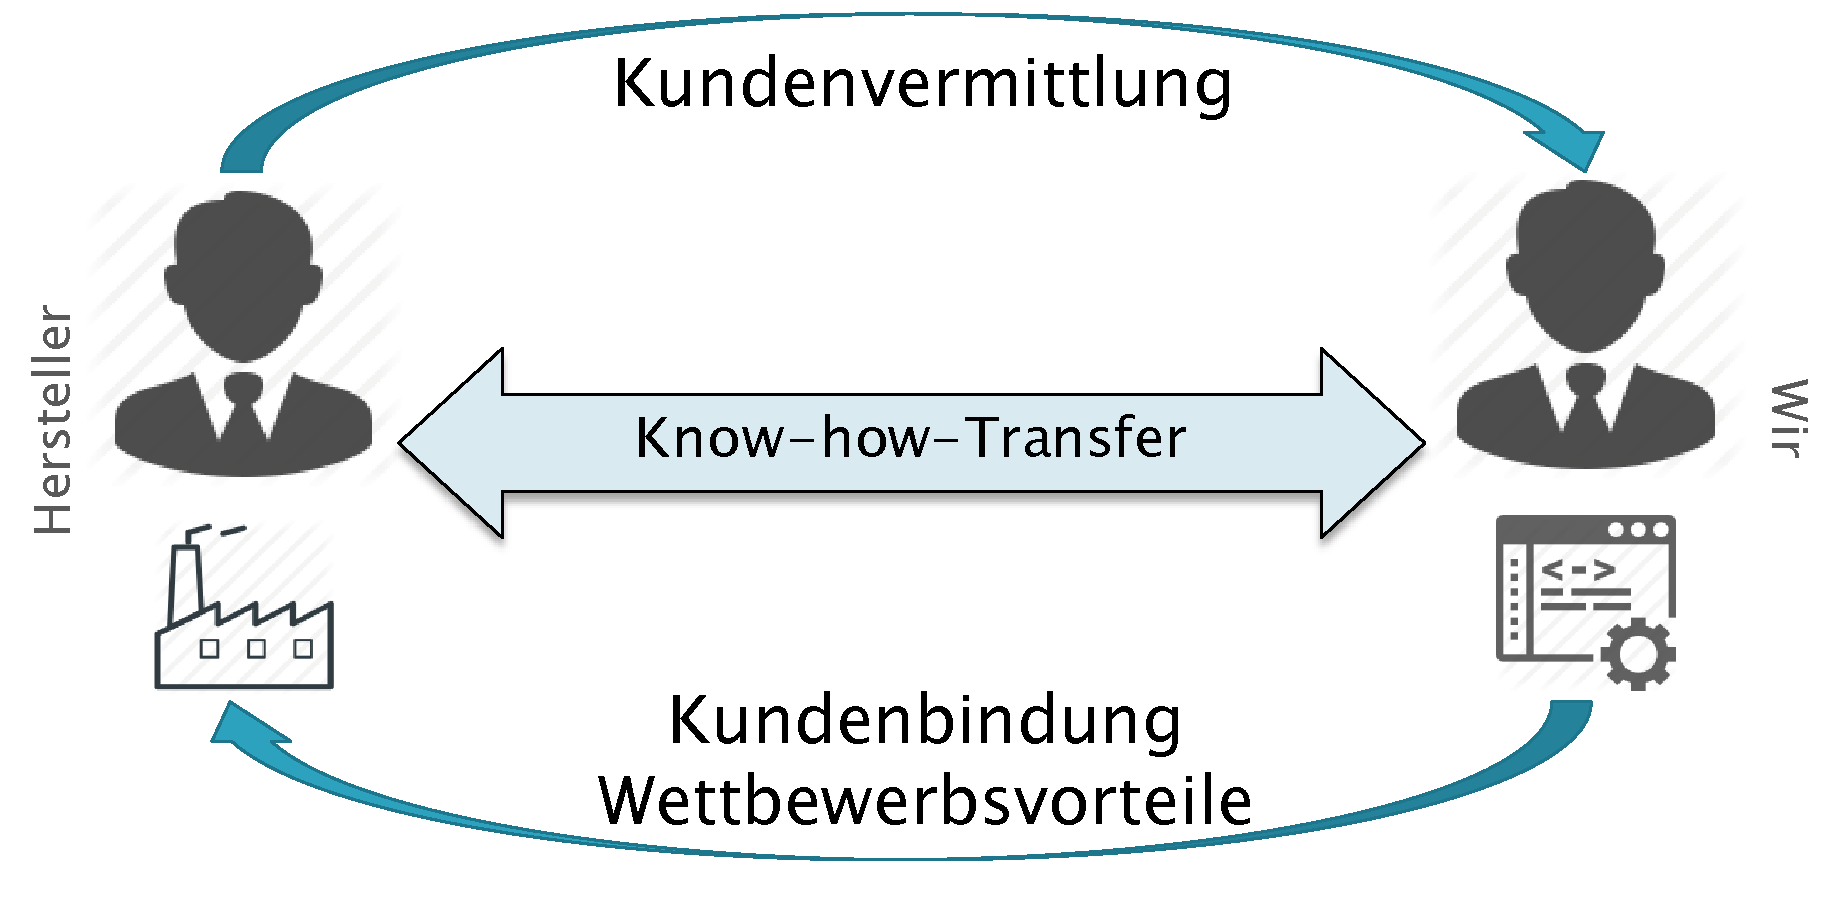
\includegraphics[width=0.7\linewidth]{Bilder/Kundengewinnung}
\caption{Strategie zur Kundengewinnung}
\label{fig:Kundengewinnung}
\end{figure}